\section{Tangent Spaces}
``What is the velocity of a curve $\gamma$ at a point $p$?''
\subsection{Velocities, Tangent Spaces}
\begin{defn}[Velocity]
    \label{defn:velocity}
    $(\mathcal{M,O,A})$ smooth manifold, curve $\gamma: \mathbb{R}\to \M$ at least $C^1$.
    Suppose $\gamma(\lambda_0) = p$.
    The velocity $v$ of $\gamma$ at $p$ is the linear map
    \begin{align*}
        v_{\gamma, p}: C^\infty(\M) &\linearto \mathbb{R}\,,\\
        f &\mapsto v_{\gamma, p}(f)\,,
    \end{align*}
    with
    \begin{equation}
        \boxed{
        v_{\gamma,p}(f) := (f \circ \gamma)'(\underbrace{\gamma^{-1}(p)}_{\lambda_0})
    }\,,
    \label{eq:defVelocity}
    \end{equation}
    \textit{i.e.}, the directional derivative of $f$ along $\gamma$ at the point $p$
\end{defn}
\begin{note}
    Remember 
    \begin{align}
        C^\infty(\M) &= \left\{ f: \M\to\mathbb{R} | f \text{ smooth, }\right. \nonumber\\
            &(f+g)(p):= f(p) + g(p)\\
            &\left.(\lambda \cdot g)(p) := \lambda \cdot g(p), \lambda \in \mathbb{R}\right\}\nonumber
    \end{align}
    is a vector space.
\end{note}
Since $f\circ\gamma: \mathbb{R}\to\mathbb{R}$ we can simply take the normal derivative.
\begin{center}
\begin{tikzpicture}
\matrix (m) [matrix of math nodes,row sep=3em,column sep=4em,minimum width=2em]
{
    \mathbb{R} & M & \mathbb{R} \\
};
\path[-stealth]
    (m-1-1) edge node [above] {$\gamma$} (m-1-2)
    (m-1-2) edge node [above] {$f$} (m-1-3)
    (m-1-1) edge[bend left = -60] node [above] {$f\circ\gamma$} (m-1-3);
\end{tikzpicture}
\end{center}
\begin{note}
    In differential calculus one had the directional derivative as $v^i(\partial_i f)$.
    The shift in philosophy is now to see $v^i\partial_i$, \textit{i.e.}, the operator
    that acts on $f$, as the vector.
\end{note}
\begin{defn}[Tangent space]
    $\forall p \in \M$ the ``tangent space to $\M$ at $p$'' consists of all the velocities
    of curves at that point :
    \begin{equation}
        \T_p\M:=\left\{ v_{\gamma,p} | \gamma\text{ smooth curves} \right\}\,.
    \end{equation}
    \label{def:tangentspace}
\end{defn}
\begin{note}
    There is no reference to any external space or embedding in definition~\ref{def:tangentspace},
    see also figure~\ref{fig:tangentspace}!
\end{note}
$\T_p\M$ can be made into a vector space. The proof for this is so important and contains so many
important things, that one should go through it in detail.

\begin{figure}[tbh]
    \centering
    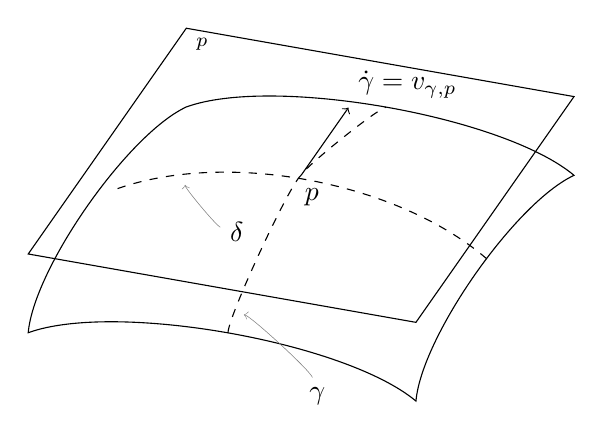
\begin{tikzpicture}[x={(170:1cm)},y={(55:.7cm)},z={(90:1cm)}]
        \draw (2.5,-2.5,0)  -- (2.5,2.5,0) node[below right] {$\T_p\M$} -- (-2.5,2.5,0) -- (-2.5,-2.5,0) -- cycle;
        \draw[looseness=.6] (2.5,-2.5,-1) node[above right] {$\M$}
        to[bend left] (2.5,2.5,-1)
        to[bend left] coordinate (mp) (-2.5,2.5,-1)
        to[bend right] (-2.5,-2.5,-1)
        to[bend right] coordinate (mm) (2.5,-2.5,-1)
        -- cycle;
        \draw[dashed,looseness=.2] (mm) to[bend left] (0,0,0) to[bend left] (mp);
        \draw[dashed,looseness=.8] (2,-0.9,0) to[bend left] (-2.8,-1,0);% to[bend left] (mp);
        \path[looseness=.2] (mm) to[bend left]
        node[pos=.2,pin={[pin distance=1cm,pin edge={solid,<-}]below right:$\gamma$}] {} (0,0,0);
        \path[looseness=.2] (2,-0.3,0) to[bend right]
        node[pos=.2,pin={[pin distance=0.5cm,pin edge={solid,<-}]below right:$\delta$}] {} (-2.8,0,0);

        \draw[->] (0,0,0) -- (0,1.5,0) node[above right] {$\dot{\gamma} = v_{\gamma, p}$};
        \node at (-0.3,-0.4,0) {$p$};
    \end{tikzpicture}
    \caption{Picture for immagining the tangent space. Keep in mind that there is no embedding needed like
    in this picture. Also in one can only think of $v_{\gamma,p}$ as an arrow in the chart, but not at
    manifold level. Also it is usefull to think of the arrow as the directional derivative $\partial_v$ in
    the direciton of this arrow. Picture adapted from~\cite{texstackexchange:tangentspace}}
    \label{fig:tangentspace}
\end{figure}
\begin{defn}[Addition and multiplication for tangent space]
    For $p\in\M$, $\gamma$ smooth curve on $\M$, $\alpha \in \mathbb{R}$:
    \begin{align}
        +:~ &\T_p\M\times \T_p\M \to \mathrm{Hom}(C^\infty(\M), \mathbb{R}) \nonumber\\
        &(v_{\gamma,p} + v_{\delta, p})(f) := v_{\gamma, p}(f) + v_{\delta, p}(f)\\
        & f \in C^\infty(M)\nonumber\\
        \cdot:~& \mathbb{R} \times \T_p\M \to \mathrm{Hom}(C^\infty(\M), \mathbb{R}) \nonumber\\
        & (\alpha \cdot v_{\gamma, p})(f) = \alpha \cdot v_{\gamma, p}(f)
    \end{align}
\end{defn}
But do they close, \textit{i.e.}, is the tangent space a vector space?
It remains to be shown that
\begin{enumerate}
    \item $\exists\, \text{curve }\sigma: v_{\gamma, p} + v_{\delta, p} = v_{\sigma, p}$
        \label{item:addofcurves}
    \item $\exists\, \text{curve }\tau: \alpha\cdot v_{\gamma,p} = v_{\tau, p}$
\end{enumerate}
The problem for~\ref{item:addofcurves} is that one cannot define $v_{\gamma,p} + v_{\delta, p}$
as just adding the points of the curves, since there is no such thing as adding two points on 
a manifold (what would be Paris + Berlin?).\\
\begin{proof} (Tangent space is a vector space)\\
    \begin{itemize}
        \item[2.]
            Construct $\tau: \mathbb{R} \to \M$:
            \begin{equation}
                \tau(\lambda) := \gamma(\alpha\cdot\lambda + \lambda_0) = (\gamma\circ\mu_\alpha)(\lambda)\,
            \end{equation}
            with $\mu_\alpha: \mathbb{R}\to\mathbb{R}, r\mapsto \alpha r + \lambda_0$.
            Then $\tau(0) = \gamma(\lambda_0) = p$.
            \begin{align}
                v_{\tau, p} &:= (f\circ\tau)'(0) = (f\circ\gamma\circ\mu_\alpha)'(0)\nonumber\\
                &= (f\circ\gamma)(\lambda_0)\alpha = \alpha v_{\gamma,p}\,.
            \end{align}
        \item [1.] Two curves $\gamma(\lambda), \delta(\lambda)$ with $\gamma(\lambda_0) = p$ and
            $\delta(\lambda_1) = p$. 
            Make a choice of chart $(U, x)$ with $p\in U$, later show independence of chart.
            Define
            \begin{align}
                \sigma_x&:\,\mathbb{R}\to\M\,,\nonumber \\
            \sigma_x(\lambda)&:= x^{-1} \left[ (x\circ\gamma)(\lambda_0 + \lambda)\right. +\\
            &+ \left.(x\circ\delta)(\lambda_1+\lambda) - (x\circ\gamma)(\lambda_0)\right]\,.\nonumber
            \end{align}
            \begin{align}
                \sigma_x(0) &= \delta(\lambda_1) = p\,,\\
                v_{\sigma_x, p}(f) &= (f\circ\sigma_x)'(0)\label{eq:vsigma}\\
                &= \left[ \underbrace{(f\circ x^{-1})}_{\mathbb{R}^d\to\mathbb{R}}\circ\underbrace{(x\circ\sigma_x)}_{\mathbb{R}^d\to\mathbb{R}} \right]'(0)\nonumber\,,
            \end{align}
            where now we use the multidimensional chain rule that a physicist would rather know as
            $\frac{\diff}{\diff \lambda}f(\vec{y}(\lambda))
            = (\vec{\nabla}_{y} f)\cdot \frac{\diff \vec{y}}{\diff\lambda}$.
            \begin{align*}
                v_{\sigma_x,p}(f) &= (x^i\circ\sigma_x)'(0)\left[\partial_i(f\circ x^{-1})\right]
                (\underbrace{x(\sigma_x(0))}_{x(p)})\\
                (x^i\circ\sigma_x)'(0) &=[(x^i\circ\gamma(\lambda_0+\lambda) + (x^i\circ\delta)(\lambda_1+\lambda)\\ 
                &~- (x^i\circ\gamma)(\lambda_0)]'\\
                &= (x^i\circ\gamma)'(\lambda_0) + (x^i\circ\delta)'(\lambda_1) = v^i_{\gamma,p} + v^i_{\delta,p}\,.
            \end{align*}
            Plugging this into equation~(\ref{eq:vsigma}) and doing the same step backwards we get
            \begin{equation}
                v_{\sigma_x, p}(f) = v_{\gamma,p}(f) + v_{\delta, p}(f)\quad\forall f\in C^\infty(\M)\,,
            \end{equation}
            independent of the chart.
    \end{itemize}
    \begin{note}
        It turns out that the sum of curves like this depends on the chart $(U, x)$, but the derivative
        of the sum of the curves at the point $p$ does not.
    \end{note}
\end{proof}
    
\subsection{Components of vectors}
Let $(U,x) \in \mathcal{A}_\text{smooth}$,
\begin{align}
    v_{\gamma,p}(f):&= (f\circ\gamma)'(0) = \left[ (f\circ x^{-1})\circ(x\circ\gamma) \right]'(0) \nonumber\\
    &= (x^i\circ\gamma)' (0) \cdot \left( \partial_i (f\circ x^{-1}) \right)\left( x(p) \right)\nonumber\\
    &=:\dot{\gamma}^i_x(0) \left(\frac{\partial f}{\partial x^i}\right)_p
    \label{eq:vectorcomponents}
\end{align}
\begin{note}
    The last step in equation~(\ref{eq:vectorcomponents}) is pure notation.
    If one sees $(\partial f / \partial x^i)_p$, one should first think of
    $\left( \partial_i (f\circ x^{-1}) \right)\left( x(p) \right)$ and also
    for $\dot{\gamma}^i_x(x)$.
    \begin{align}
        \Aboxed{%
            \left( \frac{\partial f}{\partial x^i} \right)_p &:= \left( \partial_i(f\circ x^{-1} \right)(x(p))}\,,\\
        \Aboxed{%
        \dot{\gamma}_x^i (0) &:= (x^i\circ\gamma)'(0)}\,.
        \label{eq:vectorcomponents2}
    \end{align}
    Nevertheless one can show that what we write like a partial derivative here,
    behaves (and maybe tastes) like a partial derivative.
\end{note}
Thus we write
\begin{equation}
    v_{\gamma,p}(f) = \dot{\gamma}^i_x(0)\left( \frac{\partial}{\partial x^i} \right)_p f\,,\quad\forall f\in C^\infty\,,
\end{equation}
which leads to
\begin{equation}
    v_{\gamma,p} = \underbrace{\dot{\gamma}^i_x(0)}_{\text{components}} 
\underbrace{\left( \frac{\partial}{\partial x^i} \right)_p}_{\substack{\text{chart induced} \\\text{basis of } \T_pU}}\,.
\end{equation}
\begin{theorem}[Chart induced basis of $\T_pU$]
    Let $(U,x) \in \mathcal{A}_\text{smooth}$.
    The
    \begin{equation}
        \left( \frac{\partial}{\partial x^1} \right)_p, \ldots, \left( \frac{\partial}{\partial x^d} \right)_p \quad \in \T_p\M
    \end{equation}
    constitute a \textit{basis} of $\T_pU$.
\end{theorem}
\noindent
\begin{proof}
    Show linear independence 
    \begin{align}
        \lambda^i\left( \frac{\partial}{\partial x^i} \right)_p &\stackrel{!}{=} 0\\
        \lambda^i\left( \frac{\partial}{\partial x^i} \right)_p (x^j) &= 
        \lambda^i \overbrace{\partial_i(x^j\circ x^{-1})}^{\delta_i^j}(x(p)) \nonumber\\
        &= \lambda^j\,,\quad\forall j = 1,\ldots,d\,,
    \end{align}
\end{proof}
\begin{corollary}
    \begin{equation}
        \underbrace{\mathrm{dim}\T_p\M}_{\substack{\text{vector space}\\\text{dimension}}} = d = 
        \underbrace{\mathrm{dim}\M}_{\substack{\text{top. manif.}\\ \text{dimension}}}\,.
    \end{equation}
\end{corollary}
\subsection{Change of vector components under a change of charts}
\begin{note}
    A vector is an abstract object and does not change under a change of charts.
    How should it? It does not depend on the chart.
    If it would, we could change objects by looking at them differently (different coordinates),
    so we could do telekinesis.

    What does change are the components of a vector.
\end{note}
\begin{terminology}
    $X\in \T_p\M$ always means that 
    \begin{itemize}
        \item $\exists\,\gamma:\mathbb{R}\to\M$ s.t.\ $X = v_{\gamma,p}$.
        \item $\exists\, X^1,\ldots,X^d \in \mathbb{R}: X = X^i\left( \partial/\partial x^i \right)_p$.
    \end{itemize}
\end{terminology}
Let $(U, x)$ and $(V,y)$ be overlapping charts and $p\in U\cup V$.
Let $X \in \T_p\M$.
\begin{align}
    X &= X_{(x)}^i\left( \frac{\partial}{\partial x^i} \right)_p\nonumber\\
    &= X_{(y)}^i\left( \frac{\partial}{\partial y^i} \right)_p
    \label{eq:vectransformdef}
\end{align}
Again we have to translate the ``partial derivative''-notation:
\begin{align}
    \left( \frac{\partial}{\partial x^i} \right)_p f &= 
    \partial_i \left( f\circ x^{-1} \right)(x(p))\label{eq:changeofcomp-calc}\\
    &= \partial_i \left( \underbrace{(f\circ y^{-1})}_{\mathbb{R}^d\to\mathbb{R}}
    \circ \underbrace{(y\circ x^{-1})}_{\mathbb{R}^d\to\mathbb{R}^d}
    \right)(x(p))\nonumber\,,
\end{align}
and with the multidimensional chain rule, which a physicist would write as
\begin{equation}
    \frac{\partial}{\partial x^i}\left( f(\vec{y}(\vec{x})) \right) = 
    \left( \vec{\nabla}_y f(\vec{y}) \right)\cdot \frac{\partial \vec{y}}{\partial x^i}\,,
\end{equation}
equation~(\ref{eq:changeofcomp-calc}) becomes
\begin{align}
    \left( \frac{\partial}{\partial x^i} \right)_p f &= 
    \left( \partial_i (y\circ x^{-1} )^{j}\right)(x(p))\cdot
    \left( \partial_j(f\circ y^{-1}) \right)(y(p))\nonumber\\
            &= \left(\frac{\partial y^j}{\partial x^i}\right)_p \cdot \left(\frac{\partial}{\partial y^j}\right)_p f\,.
\end{align}
Comparison with equation~(\ref{eq:vectransformdef}) yields the transformation for vector components.
Namely the components of $X$ in the $y$-chart, $X^{j}_{(y)}$ can be calculated from the components
in the $x$-chart, $X^i_{(x)}$ through
\begin{equation}
    \boxed{%
    X^j_{(y)} = \left( \frac{\partial y^j}{\partial x^i} \right)_p X^{i}_{(x)}
}\,.
\end{equation}

\subsection{Cotangent spaces}
The cotangent space of $\T_p\M$ is
\begin{equation}
    (\T_p\M)^* := \left\{ \phi: \T_p\M \linearto \mathbb{R} \right\}\,.
\end{equation}
One often just writes $\T_p\M^*$.
\begin{exmp}[Gradient]
    For $f\in C^\infty(\M)$, define 
    \begin{align}
        (\diff f)_p: \T_p\M &\linearto \mathbb{R}\nonumber\\
        X &\mapsto (\diff f)_p(X) := Xf\,,
        \label{eq:differential}
    \end{align}
    then $(\diff f)_p(X) \in \mathbb{R}$, thus
    $(\diff f)_p \in \T_p\M^*$ and we call $(\diff f)_p$ the \textit{gradient} of $f$ at $p\in M$. 
    Note that the gradient is a $(0,1)$-tensor, a covector, and not a $(1,0)$-tensor,
    which would be a vector.

    The components of the gradient with respect to the chart induced basis are
    (choosing a chart $(U, x)$)
    \begin{align}
        \nonumber \left( (\diff f)_p \right)_j &:= (\diff f)_p\left( \frac{\partial}{\partial X^j} \right)
        = \left( \frac{\partial f}{\partial x^j} \right)_p\\
        &= \partial_j (f\circ x^{-1})(x(p))\,.
    \end{align}
\end{exmp}

\begin{theorem}[Chart induced basis for the cotantent space]
    Consider chart $(U,x)$, $x^i: U \to \mathbb{R}$.
    Then
    \begin{equation}
        \left( \diff x^1 \right), \left( \diff x^2 \right), \ldots, \left( \diff x^d \right),\,,
    \end{equation}
    is a basis of $\T_p\M^*$. In fact, if one chooses the chart induced basis in $\T_p\M$,
    it is the dual basis of the dual space $\T_p\M^*$, \textit{i.e.},
    \begin{equation}
        (\diff x^a)_p \left( \frac{\partial}{\partial x^b} \right) = \delta^a_b\,.
    \end{equation}
\end{theorem}
Again, one can calculate how the components of a covector behave under a \textit{change of chart}.
Of a covector $\omega \in \T_p\M^\star$ the components are given by
\begin{equation}
    \omega = \omega_{(x)i}(\diff x^i)_p = \omega_{(y)i}(\diff y^i)_p\,,
    \label{eq:1form}
\end{equation}
Since $\omega$ is a 1-form it always acts on a vector $v\in \T_p\M$,
\begin{equation}
    \omega(v) = \omega_{(x)i}\left( \diff x^i \right)_p(v) = \omega_{(x)i}v(x^i)\,.
\end{equation}
Take a curve $\gamma(\lambda)$ for which $v$ is the tangent vector at $p$, then
\begin{align}
    \nonumber v(x^i) &= (x^i\circ \gamma)'(0) = \left( (x^i \circ y^{-1} ) \circ ( y \circ \gamma ) \right)'(0) \\
   \nonumber &= \left[ \partial_j(x^i \circ y^{-1} (y(p)) \right] \frac{\diff( y^j \circ \gamma)}{\diff \lambda}(0) \\
      \nonumber  &= \left( \frac{\partial x^i}{\partial y^j} \right)_p (y^j \circ \gamma)'(0)\\
        &= \left( \frac{\partial x^i}{\partial y^j} \right)_p v(y^j)\,.
\end{align}
Plugging this in equation~(\ref{eq:1form})
\begin{align}
    w(v) &= w_{(x)i}\left( \diff x^i \right)_p = \omega_{(x)i} \left( \frac{\partial x^i}{\partial y^j} \right)_p \left( \diff y^i \right)_p\nonumber \\
    &= w_{(y)i}\left( \diff y^i \right)_p\,.
\end{align}
So the transformation for the components of a 1-form is
\begin{equation}
    \boxed{%
        \omega_{(y)i} = \left( \frac{\partial x^j}{\partial y^i} \right)_p \omega_{(x)j}
}\,.
\end{equation}

\subsection{Bundles and Vector Fields}
Up until now we were always working at a single point $p\in \M$.
The vectors and tensors we defined live in the tangent space at that point, $\T_p\M$.
\begin{defn}[Bundle]
    A \textit{bundle} is a triple
    \begin{equation}
        \mathcal{E} \xrightarrow{\phantom{asfd}\pi\phantom{asdf}} \M\,,
    \end{equation}
    where
    \begin{itemize}
        \item $\mathcal{E}$: smooth manifold (``total space''),
        \item $\pi$: surjective smooth map (``projection map''),
        \item $\M$: smooth manifold (``base space'').
    \end{itemize}
\end{defn}
\begin{defn}[Fibre]
    $\mathcal{E} \xrightarrow{\pi} \M$ a bundle, $p\in\M$, then
    \begin{equation}
        \mathrm{preim}_\pi({p})
    \end{equation}
    is called the \textit{fibre over} $p$.
\end{defn}
\begin{defn}[Section of a bundle]
    \label{def:section}
    A \textit{section} $\sigma$ of a bundle is a map $\M\to\mathcal{E}$
    with $\pi\circ\sigma = \mathrm{Id}_\M$, \textit{i.e.}\
    a section projects a point from the base space to a point in the total space
    that is in the same fibre.
\end{defn}
\begin{center}
\begin{tikzpicture}
    \matrix (m) [matrix of math nodes,row sep=3em,column sep=4em,minimum width=2em]
    {%
        \mathcal{E}\\
        \mathcal{M}\\
    };
    \path[-stealth]
        (m-1-1) edge node [right] {$\pi$} (m-2-1)
        (m-2-1) edge [bend right = 50] node [right] {$\sigma$} (m-1-1);
        %(m-1-2) edge node [above] {$f$} (m-1-3)
        %(m-1-1) edge[bend left = -60] node [above] {$f\circ\gamma$} (m-1-3);
\end{tikzpicture}
\end{center}
\begin{note}
In figure~\ref{fig:circletangentbundle} a picture for a specific bundle is given.
We choose $\M$ to be a circle and $\mathcal{E}$ to be a cylinder with the same radius.
Then $\pi$ can be any map $\mathcal{E}\to\M$ as long as it is surjective and smooth (it can also be $\mathcal{E}\supset U \to \M$).

One possibility for $\pi$ would be to just project the point down the cylinder to the circle.
Indeed, in this picture we can see every fibre (red line) as the tangent space $T_p\M$ at the point
$p$ on the circle $\M$. Then $\mathcal{E}$ consists of all $T_p\M$ and $\pi$ takes a vector $v\in \T_p\M$
and returns $p$.
\end{note}


\begin{figure}[tbh]
    \centering
    \begin{tikzpicture}
        %\draw (-2,-2.5) grid (3,3);
        \draw[ultra thick, blue] (0,0) circle [y radius=0.5cm, x radius=1cm];
    \foreach \t in {0,...,30}
    {%
        \pgfmathsetmacro{\s}{360/30*\t}
        \pgfmathsetmacro{\x}{cos(\s+10)}
        \pgfmathsetmacro{\y}{0.5*sin(\s+10)-2}
        \pgfmathsetmacro{\yy}{\y+4}
        \ifnum\t<15
            \scoped[on background layer]
            \draw[thick,red!50] (\x, \y) -- (\x,\yy);
        \else
            \ifnum\t=20
                \draw[thick, black] (\x, \y) -- (\x,\yy);
            \else
                \draw[thick,red] (\x, \y) -- (\x,\yy);
            \fi;
        \fi;
    }
        \node[blue] at (1.3,0) {$\mathcal{M}$};
        \node[red] at (1.8,1.5) {$\mathcal{E} = \T\M$};


        \pgfmathsetmacro{\s}{360/30*20}
        \pgfmathsetmacro{\x}{cos(\s+10)}
        \pgfmathsetmacro{\y}{0.5*sin(\s+10)-2}
        \pgfmathsetmacro{\yy}{\y+4}
        \draw (\x, \yy/2+\y/2) node[circle, fill, inner sep=1pt, label=below left :$p$] (p) {};
        \node at (\x, \yy+0.2) {$\T_p\mathcal{M}$};
    \end{tikzpicture}
    \caption{Picture for a bundle, where $\M$ is a circle and $\mathcal{E}$ a cylinder.
        We have chosen $\pi$ such that every point on the cylinder ($\mathcal{E}$) is projected
        down to the circle. This way every vertical line is a \textit{fibre}.
        For example the black vertical line is the fibre over the point $p$. 
        A way to think of this specific example for the tangent space of the
        circle is that the tangent at every point of the circle is rotated so
        to give this picture. 
        Picture modified from~\cite{texstackexchange:tangentbundlecircle}.}
    \label{fig:circletangentbundle}
\end{figure}
\begin{note}
    A section is a field and what kind of field it is depends on the choice of total space.
    In figure~\ref{fig:circletangentbundle} every fibre is a vector space, namely the tangent
    space to the circle at that point.
    The base space $\mathcal{M}$ and the total space $\mathcal{E}$ don't have to lie in the
    same space like in the picture, they don't need to have anything to do with each other.
\end{note}
\begin{note}
    The wave function $\psi: \mathcal{M}\to\mathbb{C}$ is actually a scalar field and not a function.
\end{note}

\begin{defn}[Tangent Bundle of a Smooth Manifold]
$(\mathcal{M},\mathcal{O},\mathcal{A})$ a smooth manifold.
\begin{enumerate}[label=(\alph*)]
    \item The tangent bundle is the \textit{disjoint union}
        of all the tangent spaces,
        \begin{equation}
            \T\M := \bigcupdot_{p\in\mathcal{M}}\T_p\M\,.
        \end{equation}
    \item The projection map $\pi$ projects down to the base point of the
        tangent space $T_p\M$ that the vector $X$ is in,
        \begin{align}
            \pi: \T\M &\to \M \,,\\
            X &\mapsto p,\quad p\in\M: X\in \T_p \M\,.
        \end{align}
    \item Construct the \textit{coarsest} topology on $\T\M$ such that $\pi$
        is (just) continuous (``the initial topology with respect to $\pi$''),
        which here is given by
        \begin{equation}
            \mathcal{O}_{\T\M} := \left\{ \preim_\pi(\mathcal{U}) \,|\, \mathcal{U} \in \mathcal{O} \right\}\,.
        \end{equation}
\end{enumerate}    
\begin{note}
    An element $X$ of the tangent bundle $X\in\T\M$ is of course an element of the tangent space
    at its point in the manifold:
    \begin{equation}
        X \in \T_{\pi(X)}\M\,.
    \end{equation}
\end{note}
The tangent bundle itself can be made to be a smooth manifold.
Construct a $C^\infty$-atlas on $\T\M$ from the $C^\infty$-atlas $\mathcal{A}$ on $\M$,
\begin{equation}
    \mathcal{A}_{\T\M} := \left\{ (\T\mathcal{U}, \xi_x) \,|\, (\mathcal{U},x)\in\mathcal{A} \right\}\,,
\end{equation}
where
\begin{align}
    \xi_x: \T\mathcal{U} &\to \mathbb{R}^{2\dim \M}\,,\\
    X &\mapsto \left( (x^1\circ\pi)(X), \ldots, (x^d\circ\pi)(X), \right. \nonumber \\
    &~ \left.(\diff x^i)_{\pi(X)}(X), \ldots, 
    (\diff x^d)_{\pi(X)} (X)\right)\,.
\end{align}
\end{defn}
\begin{note}
    $x$ is the chart that we have chosen.
    $X \in \T\M$ is a vector in $\T_p\M$ at a base point $p$.
    We can get the base point $p$ through the map $\pi$, $p = \pi(X)$.
    The first part of $\xi_x$ are the coordinates of the base point in the chart $x$, \textit{i.e.}\ $(x\circ\pi)(X)$
    and the second part are the components of the vector which we can get by acting with $(\diff x)_{\pi(X)}$ on $X$,
    since
    \begin{equation}
        X =: X^i_{(x)} \left( \frac{\partial}{\partial x^i} \right)_{\pi(X)}\,,
    \end{equation}
    and
    \begin{equation}
        \left( \diff x^j \right)_{\pi(X)} \left( \frac{\partial}{\partial_i} \right)_{\pi(X)} = \delta^j_i\,.
    \end{equation}
\end{note}
Let's write the components of $\xi_x{X}$ as
\begin{equation}
    (\underbrace{\alpha^1, \ldots, \alpha^d}_{\text{coordinates in chart }x},
    \underbrace{\beta^1,\ldots,\beta^d}_{\text{compoenents of vector in }\T_{\pi(X)}\M})
\end{equation}
The inverse of $\xi_x$
\begin{align}
    \xi_x^{-1}: \mathbb{R}^{2\dim\M} \ni \xi_x(\T\mathcal{U}) &\to \T\mathcal{U}\,,\\
    (\alpha^1,\ldots,\alpha^d,\beta^1,\ldots,\beta^d) &\mapsto \beta^i \left( \frac{\partial}{\partial x^i} \right)_{x^{-1}(\alpha^1,\ldots,\alpha^d)}\,,
    \label{eq:xiTangentBundle}
\end{align}
and of course $x^{-1}(\alpha^1,\ldots,\alpha^d)$ is just $\pi(X)$ explicitly written out.

The atlas is \textit{smooth} if the chart transition map $\xi_y\circ\xi_x^{-1}$ is smooth.
We can check that this is true by explicitly acting with $\xi_y$ on eq.~(\ref{eq:xiTangentBundle}).
Then we see that the $\alpha^i$ transform like the coordinates in a map (because they are),
\begin{equation}
    (y^j\circ x^{-1})(\alpha^1,\ldots,\alpha^d)\,,
\end{equation}
and the
$\beta^i$ transform like the components of a tangent vector (because they are),
\begin{equation}
    \beta^m \left( \frac{\partial y^j}{\partial x^m} \right) = \beta^m \partial_m(y^i\circ x^{-1})(\alpha^1,\ldots,\alpha^d)\,,
\end{equation}
The chart transition map on the manifold level, $y^i\circ x^{-1}$, is smooth by assumption,
and the derivative $\partial_m (y^i \circ x^{-1})$ is also smooth, since the derivative of $C^\infty$ is still $C^\infty$.

We can summarize all of that in one picture:

\begin{center}
\begin{tikzpicture}
    \matrix (m) [matrix of math nodes,row sep=3em,column sep=4em,minimum width=2em]
    {%
        %\mathcal{E}\\
        %\mathcal{M}\\
        \T\M &  & \M\\
        C^\infty \text{ mfd.} & C^\infty \text{ map} & C^\infty \text{ mfd.} \\
    };
    \path[-stealth]
        (m-1-1) edge node [above] {$\pi$} (m-1-3);
        %(m-1-2) edge [bend right = 50] node [right] {$\sigma$} (m-1-1);
        %(m-1-2) edge node [above] {$f$} (m-1-3)
        %(m-1-1) edge[bend left = -60] node [above] {$f\circ\gamma$} (m-1-3);
\end{tikzpicture}
\end{center}

\begin{defn}[Vector Field $\chi$]
    A \textit{smooth vector field} $\chi$ is a \textit{smooth map}
    \label{def:vectorField}
    \begin{center}
    \begin{tikzpicture}
        \matrix (m) [matrix of math nodes,row sep=3em,column sep=4em,minimum width=2em]
        {%
            \T\M & \pi\circ\chi = \mathrm{id}_\M\\
            \M \\
        };
        \path[-stealth]
            (m-1-1) edge node [right] {$\pi$} (m-2-1)
            (m-2-1) edge [bend right = 50] node [right] {$\chi$} (m-1-1);
            %(m-1-2) edge node [above] {$f$} (m-1-3)
            %(m-1-1) edge[bend left = -60] node [above] {$f\circ\gamma$} (m-1-3);
    \end{tikzpicture}
    \end{center}
\end{defn}
\begin{note}
    We needed all the sommersaults with bundles and fibres for the word \textsc{smooth} in above definition.
\end{note}

\subsection[The C infinity module of smooth vector fields]{The $C^\infty(\mathcal{M})$ Module $\Gamma(\mathrm{T}\!\mathcal{M})$}
Remember: $C^\infty$ is the collection of smooth functions and also a vector space $(C^\infty(\M), +)$ (can add functions).
One can also multiply functions, but for the multiplication $fg$ there exists only an inverse $g^{-1}$ if the function
$g$ has no zeros (And in the definition of vector space only the multiplication with the function that is zero everywhere
is excluded). Thus $(C^\infty(\M), +, \cdot)$ is a \textit{ring}.

\begin{itemize}
    \item Field: Fulfills\footnote{\textbf{C}ommutative, \textbf{A}ssociative, \textbf{N}eutral element, \textbf{I}nverse element, \textbf{D}istributive
        } (C$^+$, A$^+$, N$^+$, I$^+$, C$^\cdot$, A$^\cdot$, N$^\cdot$, I$^\cdot$, D$^+$)
    \item Ring Fulfills (C$^+$, A$^+$, N$^+$, I$^+$, C$^\cdot$, A$^\cdot$, N$^\cdot$, $\bcancel{\mathrm{I}^\cdot}$, D$^+$)
\end{itemize}

\begin{equation}
    \Gamma(\T\M) := \left\{ \chi: \T\M\to\M\,|\,\text{smooth section} \right\}\,,
\end{equation}
which means all smooth vector fields on $\M$;
a section with total space $\T\M$ and base space $\M$ is a vector field, see definitions~\ref{def:vectorField}
and~\ref{def:section}.
\begin{defn}[Set of smooth vector fields $\Gamma(\T\M)$]
\begin{align}
    (\chi + \tilde{\chi})(f) := \chi(f) + \tilde{\chi}(f)\,.
\end{align}
Watch out for the $+$ and $\cdot$ and on what spaces they operate!
\end{defn}

One can make a vector field to an $\mathbb{R}$-vector space, by allowing multiplication with real numbers,
\begin{equation}
    (\alpha \cdot \chi) (f) := \alpha \cdot \chi(f)\,,
\end{equation}
but actually we can even make more! We can allow $C^\infty(\M)$ functions instead of $\mathbb{R}$,
\begin{equation}
    (g \cdot \chi) (f) := g \cdot \chi(f)\,,
\end{equation}
where $g \in C^\infty(\M)$. 
The point is, that $C^\infty(\M)$ is only a \textsc{ring} and so we don't call it a
$C^\infty(\M)$-vector space, but $C^\infty(\M)$-module\footnote{So a vector space over a ring is a module.}!

\begin{center}
\fbox{\parbox{0.42\textwidth}{%
        The set of all smooth vector fields $\Gamma(\T\M)$ can be made into a $C^\infty$-module
    }
}
\end{center}
A module does not have all the properties of vector spaces.
A module is \textit{not guaranteed} to always have a basis!
Thus we are \textit{not} in general able to write every vector field $\chi$ as
\begin{align}
    &\chi = f^i \chi_{(i)}\,,\\
    &\chi_{(1)}, \ldots, \chi_{(d)} \in \Gamma(\T\M)\,,\quad\text{global basis}
\end{align}
Example: Every vector field on the sphere has to vanish somewhere, 
but that means at this point it cannot be used as a basis.
We can do it locally, though, \textit{i.e.}\ for subsets $\mathcal{U} \in \M$.

\subsection{Tensor Fields}
Since $\T^*\M$ is also a vector space, we can define $\Gamma(\T^*\M)$ as all smooth
covector fields, which is again a $C^\infty(\M)$-module.
\begin{defn}[$(r,s)$-tensor field $T$]
    An $(r,s)$-tensor field $T$ is a $C^\infty$, in every element  multi-linear\footnote{Addition is like always,
    but s-multiplication means multiplying with a $C^\infty$ function.}, map
    \begin{align}
        T:\, & \underbrace{\Gamma(\T^*\M) \times \cdots \times \Gamma(\T^*\M)}_r \times\nonumber\\
        & \times \underbrace{\Gamma(\T\M) \times \cdots \times \Gamma(\T\M)}_s \linearto C^\infty(M)
    \end{align}
\end{defn}
\begin{note}
    So $T$ is a map from $C^\infty(\M)$ modules to the $C^\infty(\M)$ module $C^\infty(\M)$.
    Yes, $C^\infty(\M)$ itself is a $C^\infty(\M)$ module, just like $\mathbb{R}$ is an
    $\mathbb{R}$-vector space.
    I just want to write $C^\infty(\M)$ once more: $C^\infty(\M)$.
\end{note}

Example: $f \in C^\infty(\M)$
\begin{align}
    \diff f:\,\Gamma(\T\M)&\linearto C^\infty(\M)\\
    \chi &\mapsto \diff f(\chi):= \chi f\,,
\end{align}
where $\chi f$ is defined by its action on $p\in\M$,
\begin{equation}
    (\chi f)(p) := \chi(p) f\,,
\end{equation}
which works since $\chi(p)\in\T{p}\M$ can act on a function $f$.
Thus $\diff f$ is a gradient co-vector field.

